\chapter{Grundlagen}

Das Grundlagenkapitel gibt eine Einführung und Übersicht über die verwendeten Begriffe und Konzepte, auf die im Weiteren der Arbeit zurückgegriffen wird. Zunächst wird die Darstellung von Bildern behandelt und anschließend die Erhebung von charakteristischen Merkmalen aus Bildern, den Features. Zur Detektion und Extraktion von Features aus Bildern haben sich zahlreiche verschiedene Verfahren etabliert. Von diesen wird der SIFT Feature-Detektor und Deskriptor näher betrachtet, da dieser im Weiteren als Basis für die Gewinnung der Features dient. 
Es werden anschließend zwei Modelle vorgestellt, die eine Klassifikation von Bildern auf Basis von Features ermöglichen. Das Bag of Visual Words Modell wurde aus dem Bereich Information Retrival adaptiert. Es wird anhand der Features von Trainingsbildern ein visuelles Vokabular gelernt, das zur Klassifizierung von Bildern dient. Alternativ zu diesem Ansatz wird der Autoencoder vorgestellt. Ein Autoencoder ist ein spezielles neuronales Netzwerk, das selbständig eine komprimierte Darstellung der Eingabe, in diesem Fall der Features, lernt. 
Im letzten Teil wird auf die Berechnung allgemein mathematischer Probleme auf Grafikkarten, das GPU Computing eingegangen. Durch den Einsatz von Grafikkarten können Berechnungen gerade bei großen Datenmengen stark beschleunigt werden, da diese massiv parallel auf den Daten arbeiten. Mit Nvidias CUDA wird ein Ausführungsmodell eingeführt, mit der sich Modelle wie der Bag of Visual Words und Autoencoder auf Nvidia Grafikkarten ausführen lassen.

\section{Bilder und Features}

Zunächst wird definiert wie ein Bild mathematisch aufgefasst wird, um eine effiziente Verarbeitung zu ermöglichen. Jedes Verfahren erwartet ein Bild als Eingabe. Verändern Algorithmen ein Bild, so geben sie die bearbeite Version wieder aus. Bei Analysen hingegen wird ein Bild nicht verändert, es wird auf Muster untersucht und die gefundenen Eigenschaften zurückgegeben. Diese Eigenschaften werden Features genannt. Der Prozess der Featuregewinnung ist in Detektion und Extraktion unterteilt und wird im Anschluss behandelt.

\subsection{Bilder}

Bei einem digitalen Bild handelt es sich um eine Matrix $I(x, y)$. Die Anzahl der Spalten $m$ und Zeilen $n$ entspricht dabei den Dimensionen des Bildes in Pixeln. Hier bezeichnen $(x, y)$ Indizes der Matrix und somit die einzelnen Pixel des Bildes. Die Darstellung in Matrixform eignet sich  sehr gut für Transformationen und Analysen des Bildes. Solche Verfahren betrachten oft jeden Pixel und seine Nachbarschaft. \todo{Ändern} Die direkte Nachbarschaft eines Pixels ist eine $3 \times 3$ Matrix (mit dem Pixel als Zentrum), die alle unmittelbar anliegenden Pixel beinhaltet.

$$
I(x, y) = \begin{bmatrix}
i_{0, 0}   & i_{0, 1}	& \dots	 & i_{0, n-1}   \\
i_{1, 0}   & i_{1, 1}   & \dots  & i_{1, n-1}   \\
\vdots	   & \vdots 	& \ddots & \vdots       \\
i_{m-1, 0} & i_{m-1, 1} & \dots	 & i_{m-1, n-1}
\end{bmatrix}
$$ 

Abhängig vom Typ des Bildes, besitzen die Pixel eine andere Struktur. In der Bilderverarbeitung und im Weiteren dieser Arbeit werden meist folgenden Arten von Bildern verwendet:
\begin{itemize}
	\item \textbf{Monochromatische Bilder} Diese Bilder werden nur in Graustufe dargestellt, daher besitzt ein Pixel genau einen Intensitätswert.
	\item \textbf{Multispektrale Bilder} Jeder Pixel besitzt einen Vektor an Werten. Im Falle eines Farbbildes enthält der Vektor drei Intensitätswerte für rot, grün und blau.
\end{itemize}
Die Intensität eines Pixels bzw. die Intensität seiner Vektoren wird mit acht Bit dargestellt und umfasst daher 256 mögliche Werte. Diese Werte werden im Folgenden normalisiert im Intervall $[0, 1]$ angegeben. 

\subsection{Feature Detektion und Extraktion}

Um Bilder zu vergleichen werden charakteristische Merkmale dieser betrachtet, die sogenannten Features. Ein Feature ist ein allgemeiner Begriff und enthält je nach Verfahren unterschiedliche Informationen. Dies ist notwendig, da nicht nur die Position oder Intensität eines Pixels, sondern auch generelle Eigenschaften von Interesse sind. Globale Verfahren berücksichtigen bei der Bewertung jeden Pixel des Bildes gleichermaßen, lokale hingegen betrachten nur ein kleine Fenster des Bildes, also einen Pixel und seine Nachbarschaft. Die Suche nach globalen Merkmalen, die ein Bild charakterisieren, kann aber keine Objekte und Details im Bild berücksichtigen. Hierfür eignet sich die Extraktion von lokalen Features. Um Objekte aus unterschiedlichen Perspektiven und in verschiedenen Größen wieder zu erkennen, ist es notwendig, dass die Features affin invariant sind. Abbildung \ref{img:liberty} zeigt dasselbe Objekt, jedoch rotiert, skaliert und verschoben. Ein Algorithmus sollte mit hoher Wahrscheinlichkeit erkennen, dass es sich hier um dasselbe Objekt handelt.

\begin{figure}
	\centering
	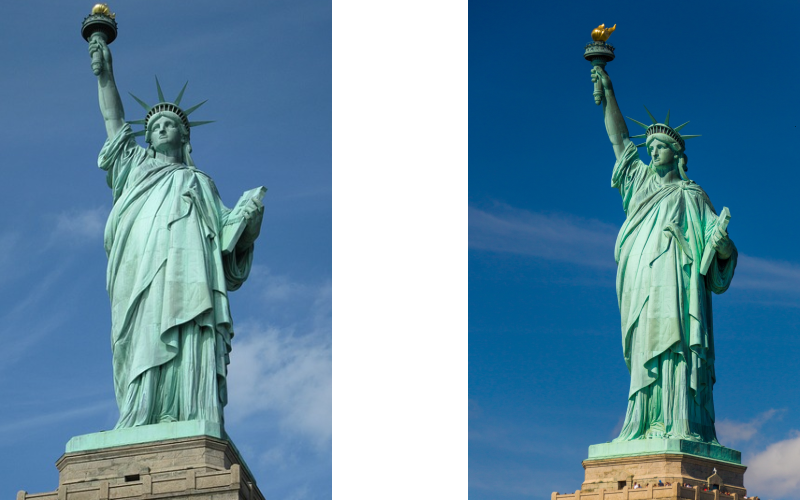
\includegraphics[scale=0.55]{images/liberty.png}
	\caption{Zwei Bilder mit dem gleichen Objekt aus unterschiedlicher Perspektive und in verschiedenen Lichtverhältnissen.}
	\label{img:liberty}
\end{figure}

Die Gewinnung der Features ist in zwei Schritte aufgeteilt: 
\begin{itemize}
	\item \textbf{Detektion} Zuerst ermittelt ein Detektor Muster im Bild. Die untersuchten Muster sind abhängig vom Detektor Pixel, Linien oder Regionen einer Nachbarschaft. Hierfür wird jeder Pixel und seine Nachbarschaft betrachtet und entschieden ob es sich um einen \textit{keypoint} handelt. Ein Detektor gibt als Ergebnis alle Pixel zurück, bei denen es sich um \textit{keypoints} handelt. Manche Verfahren geben zusätzlich zu den \textit{keypoints} auch Eigenschaften wie die Orientierung oder den Maßstab aus. Um praktisch einsetzbar zu sein, muss ein Detektor ein Feature, dass in verschiedenen Bildern auftaucht, zuverlässig erkennen. Hier sollte aber die angestrebte Allgemeinheit berücksichtigt werden: Ein Feature Detektor für medizinische Bilder kann speziellere Annahmen treffen, als einer für eine allgemeine Bildsuche.
	\item \textbf{Extraktion} Die Feature Extraktion erzeugt aus den vom Detektor gefundenen \textit{keypoints} den Deskriptor. Ein Feature-Deskriptor ist eine kompakte Darstellung eines Features. Die \textit{keypoints} und deren Eigenschaften werden in Zahlen kodiert. Oft wird hier nicht nur ein Feature erzeugt, sondern ein Feature-Vektor, der auch Deskriptoren der Nachbarschaft des \textit{keypoints} enthält. Von einem Deskriptor ist es wünschenswert, dass er affin invariant ist. Somit kann das Feature auch erkannt werden, wenn das Bild rotiert, verschoben oder skaliert wurde. \todo{Affine Invarianz?}
\end{itemize}

Im Folgenden werden zwei Verfahren zur Feature Detektion und Extraktion vorgestellt, die sich in der Praxis bewährt haben und teilweise affine Invarianz aufweisen. Das Histogram of Oriented Gradients ist ein weit verbreiteter Feature Deskriptor, der sich im Bereich der Objektdetektierung bewährt hat. SIFT ist ein von Lowe \cite{dif2004} entwickeltes Verfahren zur Feature Extraktion und Detektion. Bei der Detektion von Features werden Rotationen, Skalierungen und Translationen von gefundenen Features erkannt und diese durch den Deskriptor als ein Histogramm der Orientierungen dargestellt.\cite{ifd2016}

\begin{figure}
	\centering
	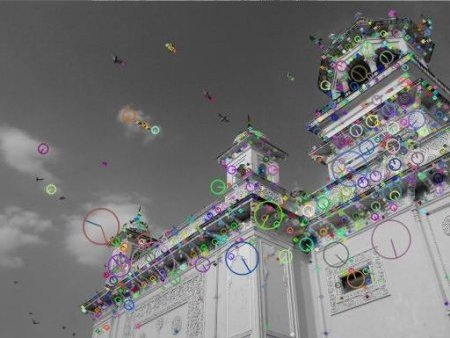
\includegraphics[scale=0.7]{images/sift_keypoints.jpg}
	\caption{Gefundene \textit{keypoints} in einem Bild farblich hervorgehoben (SIFT Detektor)}
	\label{img:interset_points}
\end{figure}

\subsection{Histogram of Oriented Gradients}

Ein Histogramm ist eine diskrete Funktion, welche die Häufigkeitsverteilung in einer Menge abbildet. Hierfür wird jeder Wert der Menge einer Klasse zugeordnet. Die Größe der Intervalle einer Klasse leiten sich aus der Größe des gesamten Wertebereichs und der Anzahl der Klasse ab. So kann beispielsweise die Verteilung der Pixel eines Bildes auf die Intensitäten als Histogramm betrachtet werden. Bei einem monochromatischen Bild liegen 256 Intensitätswerte vor, die je eine Klassen repräsentieren. Beim Bilden des Histogramms wird jeder Pixels betrachtet und der Zähler der Klasse um eins inkrementiert, in deren Wertebereich der Intensitätswert des Pixels fällt. Ein Histogramm ist normalisiert, wenn es die relative Verteilung in der Menge darstellt.
In Abbildung \ref{img:hist} sind im Wesentlichen zwei Bereiche zu erkennen: ein sehr heller Hintergrund und eine dunkle Katze, die den Großteil des Bildes ausmacht. Dies spiegelt sich auch im Histogramm wieder: Es ist eine große Mengen an Punkten im dunklen Bereich vorhanden (Intensität $< 128$) und eine kleine, extreme Häufung im hellen Bereich.

\begin{figure}
	\centering
	\includegraphics[scale=0.8]{images/big_cat.png}
	\caption{Graustufenbild und Verteilung der Intensitätswerte}
	\label{img:hist}
\end{figure}

Das Histogramm of Oriented Gradients beschreibt die Änderung der Intensität von einer Menge benachbarter Pixel in einer Richtung an. Um ein HOG zu generieren wird das Bild in gleich große Zellen eingeteilt, die eine Nachbarschaft von Pixeln umfassen. Über die Pixel jeder Zelle werden nun die lokalen Gradienten berechnet. Diese fließen proportional zu ihrer Stärke in den kumulierten Gradienten der Zelle ein. Dabei hat jede Zelle eine feste, vorgegebene Anzahl an Klassen für die Orientierungen der Gradienten. 

Dalal und Triggs \cite{hog2005} nutzten in ihrer Originalarbeit als Fenster eine 64 $\times$ 128 Nachbarschaft von Pixeln, eine Zellgröße von 8 $\times$ 8 Pixeln und $2 \times 2$ Zellen pro Block. In Abbildung \todo{Abbildung} ist links das Fenster dargestellt und rechts die entsprechenden Gradienten der Zellen. 

\todo{Abbildung}

\subsection{Scale-invariant feature transform}

SIFT ist ein Feature-Detektor und Deskriptor der 1999 von Lowe \cite{dif2004} entwickelt wurde. Neben der Invarianz der Skalierung der Features, berücksichtigt SIFT auch die Rotation, Beleuchtung und Perspektive. Der Algorithmus lässt sich in vier wesentliche Schritte unterteilt:

\begin{enumerate}
	\item \textbf{Scale space} Im ersten Schritt wird die Invarianz der Skalierung behandelt. SIFT konstruiert hierfür einen \textit{scale space}. Hier werden aus dem Originalbild immer verzerrtere Versionen durch einen \todo{gausschen Filter} erzeugt. Die Größe der neuen Bilder wird halbiert und die Prozedur wiederholt. Alle verzerrten Bilder einer Größe bilden eine sogenannte Oktave. SIFT verwendet vier Oktaven und fünf Bilder pro Oktave um den \textit{scale space} zu erzeugen. Um Ecken und Kanten in einem Bild zu ermitteln, die Kandidaten für \textit{keypoints} sind, wird nun zwischen allen aufeinanderfolgenden Bildern einer Oktave die Differenz gebildet. Das Prinzip ist für zwei Oktaven in Abbildung \ref{img:sift_dog} dargestellt. Das Ergebnis ist eine Approximation des \todo{Laplacian of Gaussians}, jedoch ist dieses Verfahren weit weniger rechenintensiv. 

\begin{figure}
	\centering
	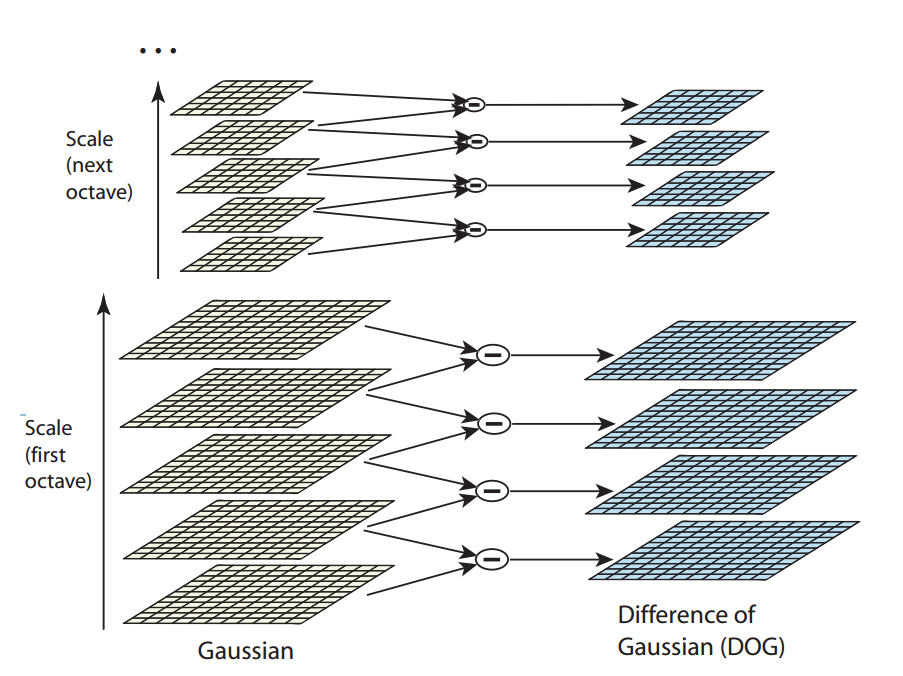
\includegraphics[scale=0.5]{images/sift_dog.png}
	\caption{Difference of Gaussians Operator \cite{dif2004}}
	\label{img:sift_dog}
\end{figure}	
	\item \textbf{Keypoint Ermittlung} Nicht alle Kandidaten werden zu \textit{keypoints}. Aus den DOG \todo{DOG erklären} Bildern werden nun die Extrempunkte bestimmt. Hierfür wird immer eine Nachbarschaft des DOG Bildes und des vorigen und nachfolgendem im \textit{scale space} betrachtet. Da die Extremwerte nicht immer exakt auf einem Pixel liegen, muss die genau Position noch berechnet werden. SIFT verwendet hierfür eine Taylor Entwicklung im angenäherten \textit{keypoint} ausgehend.
	\item \textbf{Bestimmung der Orientierung} Bei dem Aufbau des Feature Vektoren pro \textit{keypoint} wird die lokale Orientierung berechnet. Auf diese Weise sind die SIFT Deskriptoren invariant gegenüber Rotationen. Der SIFT Algorithmus berechnet ein Histogram of Oriented Gradients. Hierfür werden zufällig Punkte aus der Nachbarschaft des \textit{keypoints} ausgewählt. Der Extremwert des Histogramms wird dann als dominante Orientierung verwendet.
	\item \textbf{Deskriptor} Für jeden durch den Detektor gefundenen \textit{keypoint} wird nun ein Feature-Vektor gebildet. Der Feature-Vektor enthält Informationen über die Nachbarschaft in Form der Gradienten. Das Fenster für die Auswahl der Nachbarschaft wird auf dem \textit{keypoint} zentriert und in vier Teilfenster unterteilt. Die Gradienten in allen Teilfenster werden in acht Richtungen gemessen, sodass der resultierende Deskriptor 128 Komponenten enthält.
\end{enumerate}

SIFT ist äußerst robust, da Änderungen im Grenzwert von Position und Orientierung den Feature-Vektor kaum beeinflussen. Der Deskriptor besitzt zwar keine affine Invarianz, in praktischen Anwendungen werden jedoch auch mit skalierten, rotierten und verschobenen Objekten gute Ergebnisse erzielt. Die Konstruktion des Deskriptors ist allerdings sehr aufwendig und die Darstellung erfordert einen Raum mit 128 Dimensionen. \cite{dif2004}

\todo{SIFT-PCA erwähnen}

\section{K-means Clustering}

Unter k-means Clustering werden Algorithmen zusammengefasst, die eine Menge Vektoren durch Zuweisung in $k$ vorgegebene Gruppen einteilen, die sogenannten Cluster. Aus den Vektoren werden initial $k$ Stück ausgewählt, die als anfängliche Schwerpunkte der Cluster dienen. Ein k-means Algorithmus ordnet nun iterativ jeden Vektor dem Cluster zu, dessen Varianz sich bei Aufnahme des Vektors am Wenigsten erhöht. Aus diesem Grund setzt das k-means Clustering einen euklidischen Raum voraus.
Soll ein globales Optimum gefunden werden, so ist k-means NP-schwer. Praktische Implementierungen approximieren daher meist die Schwerpunkte der Cluster, wie beispielsweise der Algorithmus von Llyod. Zunächst beginnt Llyods Algorithmus mit einer Initialisierung der Schwerpunkte. Schritt zwei und drei werden dann solange wiederholt, bis der Algorithmus konvergiert, also die Vektor-Cluster-Zuordnung sich nicht mehr oder nur noch gering ändert oder eine maximale Anzahl an Iterationen erreicht wurde: 

\begin{enumerate}
	\item \textbf{Initialisierung} Es werden zunächst $k$ zufällige Vektoren als Schwerpunkte der Cluster ausgewählt.
	\item \textbf{Zuordnung}: Von den verbleibenden Vektoren wird nun mit jedem Cluster die neue Summe der Varianzen bei Aufnahme des Vektors berechnet. Es wird der Vektor dem Cluster zugeordnet, dessen Varianz sich am geringsten bei Aufnahme des Vektors erhöht.
	\item \textbf{Vektoren zuweisen}: Die Zentren den Cluster werden neu berechnet, um den neu zugeordneten Vektor in Folgeberechnungen miteinzubeziehen.
\end{enumerate}

Zur geometrischen Veranschaulichung sind in Abbildung \ref{img:bovw} Punkte im zweidimensionalen Raum gegeben. Die Verteilung der Punkte ist in diesem Beispiel idealisiert, um bei einem Clustering mit einem $k = 3$, die Cluster in der rechten Grafik zu erhalten. Dies illustriert auch, dass abhängig von den Daten nicht immer sinvolle Cluster gebildet werden können. \cite{mmd2011}

\begin{figure}
	\centering
	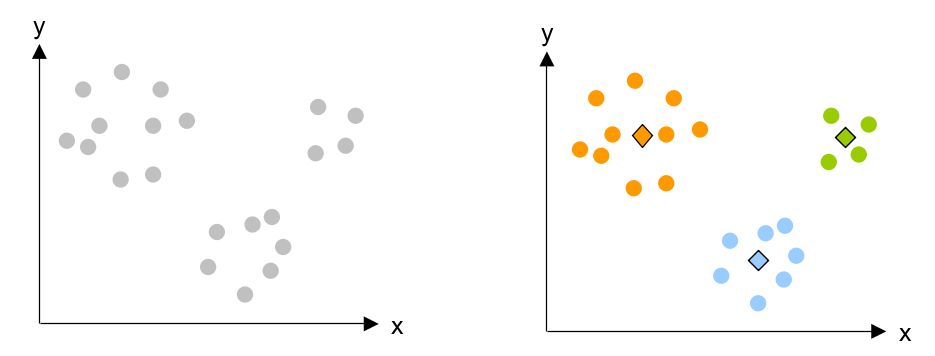
\includegraphics[scale=0.55]{images/kmeans.png}
	\caption{K-means Clustering im zweidimensionalen Raum mit $k = 3$.}
	\label{img:bovw}
\end{figure}

\section{Bag of Visual Words}

Das Bag of Words Modell stammt aus dem Bereich Information Retrival und wird zur Klassifizierung von Dokumenten genutzt. Es wird das Auftreten jedes Wortes in einem Dokument gezählt und durch die Anzahl aller Wörter im Vokabular dividiert, um so einen normalisierten Wert zu erhalten, welcher die relative Häufigkeit eines Wortes angibt. Das Vokabular wird \textit{Codebook} genannt, die Wörter sind die \textit{Codewords}.
Dieses Modell wurde von der Computer Vision adaptiert um Bilder zu klassifizieren. Die Features können aber nicht direkt statt der Worthäufigkeit verwendet werden: Ein Wort ist ein diskreter Wert der direkt verglichen werden kann, ein Feature hingegen ist ein Vektor in einem hochdimensionalen Raum, der Eigenschaften beschreibt. Um konkrete Werte zu erhalten, ist es notwendig, die Vektoren zu quantisieren. Die quantisierten Vektoren entsprechen dann den \textit{Codewords} und werden in diesem Kontext auch \textit{Visual Words} genannt. Um \textit{Visual Words} aus einer Menge von Trainingsbildern zu erhalten, werden zunächst Feature-Vektoren aus den Bildern extrahiert. Die Features werden dann durch ein Clusteringverfahren gruppiert. Die Idee ist, dass ähnliche Vektoren nah beieinander im Raum liegen und somit in die gleiche semantische Kategorie gehören. Durch einen Clustering Algorithmus wie k-means kann die Größe des \textit{Codebooks} bestimmt werden. Wird für $k$ ein große Zahl gewählt, wird ein Vokabular von Exemplaren aufgebaut, ein kleines $k$ hingegen erkennt eher Kategorien. Die Schwerpunkte der Cluster vertreten dann eine Menge von ähnlichen Features und bilden das \textit{Codebook}.
Auf Basis des \textit{Codebooks} kann der Bag of Words von Bildern erzeugt werden. Hierfür werden wieder die Features eines Bildes extrahiert. Aus diesen Daten wird nun eine Histogrammdarstellung des Bildes erzeugt: Für jedes Feature wird das ähnlichste \textit{Visual Word} des \textit{Codebooks} bestimmt und die entsprechende Klasse inkrementiert.

\todo{Abbildung Prozess}

\todo{Quelle}

\section{Autoencoder}

Ein Autoencoder ist ein spezielles neuronales Netzwerk. Diese Netze werden für das unbeaufsichtigte Lernen einer komprimierten Darstellung von Daten genutzt. Zunächst wird hierfür ein Überblick über das Themengebiet der neuronale Netze im Allgemeinen gegeben und anschließend die Funktionsweise eines Autoencoders erläutert. Darauf aufbauend werden zwei Erweiterungen des Autoencoders vorgestellt, um Rauschen in den Daten und tiefe Netzwerke berücksichtigen.

\subsection{Neuronale Netze}

Neuronale Netze sind dem Aufbau und der Funktionsweise der Neuronen des menschlichen Gehirns nachempfunden. Es wird eine Menge von künstlichen Neuronen genutzt, um eine Lösung für ein Problem zu gestalten. Erste theoretische Überlegungen tauchten bereits in den 40er Jahren auf. Durch die wachsende Rechenleistung und neue Forschungsgebiete wie Deep Learning und Machine Learning finden neuronale Netze seit Mitte der 80er Jahre vermehrt praktische Anwendung und akademische Zuwendung. Dadurch, dass neuronale Netze von Natur aus hoch parallel arbeiten können, eignen sie sich vor allem für parallele Architekturen und die Verarbeitung großer Datenmengen. 
Ein neuronales Netz besteht aus einer Menge Neuronen, die in Schichten im Netzwerk angeordnet sind. Jedes Neuron besitzt einen Aktivierungszustand und einen Schwellwert, von denen abhängt, ob ein Signal weitergeleitet wird. Neuronen benachbarter Schichten sind vollständig durch gewichtete Kanten miteinander verbunden. Diese Beziehung wird in einer Gewichtsmatrix ausgedrückt. Eine Kante zwischen zwei Neuronen die nicht verbunden sind, hat dann den Wert 0 als Gewicht, um die Abwesenheit auszudrücken. 
Das Netz verarbeitet ein Signal, welches hier als Vektor $x \in [0,1]^n$ aus $\mathbb{R}^n$ dargestellt wird. Die erste Schicht des Netzwerks, der \textit{Input layer}, leitet das Signal nur an die nächste Schicht weiter und besitzt daher $n$ Neuronen. Die letzte Schicht, der \textit{Ouput layer}, dient zur Ausgabe des Ergebnisvektors $z \in [0,1]^m$, wobei $m$ die Anzahl der Elemente des Vektors angibt. Zwischen diesen beiden Schichten können sich beliebig viele \textit{Hidden layer} befinden. Die \textit{Hidden layer} bilden somit den Kern des Netzes, deren Kantengewichtungen, Kanten oder Neuronen während eines Lernprozess angepasst werden. In Abbildung \ref{img:nnexample} ist ein Netz mit drei Schichten dargestellt. Der \textit{Input layer} nimmt einen vierdimensionalen Vektor als Eingabe entgegen. Die Werte des Vektors werden an jedes der fünf Neuron im \textit{Hidden Layer} weitergeleitet, was durch die Kanten symbolisiert wird. Jede Kante besitzt dabei ein Gewicht, dass aus Gründen der Übersicht nicht aufgeführt ist. Schließlich werden die Ausgaben des \textit{Hidden layers} an das einzige Neuron des \textit{Output layers} geschickt und von diesem als Ergebnis $z$ ausgegeben.

\begin{figure}
	\centering

	\begin{tikzpicture}[shorten >=1pt,->,draw=black!50, node distance=\layersep]
    \tikzstyle{every pin edge}=[<-,shorten <=1pt]
    \tikzstyle{neuron}=[circle,fill=black!25,minimum size=17pt,inner sep=0pt]
    \tikzstyle{input neuron}=[neuron, fill=green!50];
    \tikzstyle{output neuron}=[neuron, fill=red!50];
    \tikzstyle{hidden neuron}=[neuron, fill=blue!50];
    \tikzstyle{annot} = [text width=6em, text centered]

    % Draw the input layer nodes
    \foreach \name / \y in {1,...,4}
        \node[input neuron, pin=left:$x_{\y}$] (I-\name) at (0,-\y) {};

    % Draw the hidden layer nodes
    \foreach \name / \y in {1,...,5}
        \path[yshift=0.5cm]
            node[hidden neuron] (H-\name) at (\layersep,-\y cm) {};

    % Draw the output layer node
    \node[output neuron,pin={[pin edge={->}]right:$z$}, right of=H-3] (O) {};

    % Connect every node in the input layer with every node in the
    % hidden layer.
    \foreach \source in {1,...,4}
        \foreach \dest in {1,...,5}
            \path (I-\source) edge (H-\dest);

    % Connect every node in the hidden layer with the output layer
    \foreach \source in {1,...,5}
        \path (H-\source) edge (O);

    % Annotate the layers
    \node[annot,above of=H-1, node distance=1cm] (hl) {Hidden layer};
    \node[annot,left of=hl] {Input layer};
    \node[annot,right of=hl] {Output layer};
	\end{tikzpicture}

	\caption{Beispiel eines dreischichtigen neuronalen Netzes.}
	\label{img:nnexample}
\end{figure}

Die Verarbeitung eines Signals in einem Neuron ist in Abbildung \ref{img:neuron} schematisch dargestellt und lässt sich in drei Schritte untergliedern:
\begin{itemize}
	\item \textbf{Propagierungsfunktion} Aus der Eingabe aller verbundenen Neuronen wird die Netzeingabe berechnet. Meist wird hier die gewichtete Summe zwischen Eingabe und Gewicht verwendet: $\sum_{i=1}^{} w_{i}x_{i} + b$.
	\item \textbf{Aktivierungsfunktion} Es wird der neue Aktivierungszustand des Neurons aus dem alten Zustand und der Netzeingabe berechnet. Häufig wird hier die \todo{logistische} Funktion $s(x) = \frac{1}{1+e^{-x}}$ verwendet.
	\item \textbf{Ausgabefunktion} Wird ein Neuron aktiviert, so wird das resultierende Signal durch die Ausgabefunktion berechnet und an alle Neuronen in der folgenden Schicht weitergeleitet. Oft wird hier die Identitätsfunktion verwendet.
\end{itemize}

\begin{figure}
	\centering
	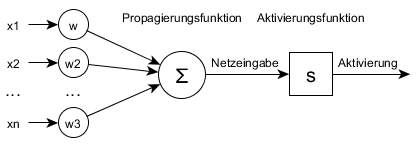
\includegraphics[scale=1.0]{images/neuron.png}
	\caption{Verarbeitung eines Signales in einem Neuron (ohne Ausgabefunktion) (Grafik überarbeiten)}
	\label{img:neuron}
\end{figure}

Wurde ein neuronales Netz konstruiert, folgt darauf die Trainingsphase. Durch das Training ist es möglich, dass ein Netzwerk Neuronen oder Verbindungen hinzufügt bzw. entfernt, den Schwellwert für die Aktivierung von Neuronen verändert oder die Gewichte zwischen Neuronen anpasst. Pro Trainingselement wird die Fehlerquote $F$ zwischen dem angestrebten Ergebnis $z'$ und der Ausgabe des Netzes $z$ berechnet:
$$ F(z, z')=\sum_{i=0}^{n}(z'_{i} - z_{i})^2 $$
Durch eine Lernregel werden abhängig von der Fehlerquote beispielsweise die Gewichte der Kanten angepasst. Für Netze ohne \textit{Hidden layer} eignet sich hier die Hebbsche oder Delta Lernregel. Für Netze mit mindestens einem \textit{Hidden layer}, hat sich das \textit{Backpropagation} Verfahren etabliert. \textit{Backpropagation} minimiert den Gradientenabstieg auf der Fehleroberfläche die $F$ aufspannt. Der Algorithmus geht in drei Schritten vor:

\begin{enumerate}
	\item \textbf{Forward Pass} Die Gewichte des Netzwerks werden initialisiert und eine Eingabe durch das Netz propagiert. Als Resultat liegt die Ausgabe vor.
	\item \textbf{Fehlerberechnung} Die Fehler des \textit{Output layers} werden, durch einen Vergleich mit den erwarteten Werten, berechnet. Falls die Fehler unterhalb einer vorgegebenen Grenze liegen, ist das Training beendet. Andernfalls wird fortgefahren.
	\item \textbf{Backward Pass} In diesem Schritt wird die Fehlerquote rückwärts durch das Netz propagiert. Die Gewichte an den Verbindungen zwischen Neuronen werden in Abhängigkeit ihres Einflusses auf den Fehler Schicht für Schicht aktualisiert.
\end{enumerate}

\todo{Gradienten erläutern}

\subsection{Funktionsweise}
Ein Autoencoder (AE) ist ein spezielles neuronales Netzwerk, dass eine komprimierte Kodierung der Eingabe lernt. Ein Autoencoder versucht die Daten zu rekonstruieren und kann daher unbeaufsichtigt lernen: Die rekonstruierten Daten können anhand einer Distanzmetrik mit den Originaldaten verglichen werden. Anschließend kann die Größe des Fehlers berechnet werden und durch \textit{Backpropagation} die Gewichtesmatrix aktualisiert werden.
Um die Originaldaten als Ergebnis erhalten zu können, muss die Anzahl der Neuronen des \textit{Input layers} der Anzahl der Neuronen im \textit{Output layer} entsprechen. Die Anzahl der Neuronen im \textit{Hiddenlayer} ist geringer, um die komprimierte Darstellung des Features zu erreichen. Werden mehrere \textit{Hiddenlayer} verwendet, so nimmt die Neuronenanzahl von Layer zu Layer ab um die Anzahl der Komponenten weiter zu verringern. Dieser Vorgang ist die Enkodierung und liefert die gewünschte komprimierte Abbildung. Die Dekodierung ist umgekehrt aufgebaut, um das Original aus der komprimierten Repräsentation Schicht für Schicht zu rekonstruieren. Wie gut die Dekodierung gelungen ist, lässt sich dann anhand eines Vergleichs der Distanz des Original und der Rekonstruktion bewerten. Formal wird ein Eingabevektor $x \in [0,1]^n$ auf einen Vektor $y \in [0,1]^p$ durch $y = encode_{W,b}(x) = s(Wx + b)$ abgebildet. $W$ ist die Gewichtsmatrix $n \times p$ und $b$ der \todo{Bias-Vektor}. Diese Parameter werden durch den Autoencoder optimiert. Die Rekonstruktion erfolgt durch die Dekodierungsfunktion: $z \in [0, 1]^n$ wird dann durch $z = decode_{W', b'}(y) = s(W'y + b')$ berechnet. \cite{ssn1997}.

In Abbildung \ref{img:example_ae} ist ein Autoencoder abgebildet der als Eingabe einen Vektor $x \in [0,1]^4$ entgegen nimmt. Dieser wird auf den Vektor $y$ mit drei Komponenten abbildet, da der \textit{Hidden layer} drei Neuronen enthält. Die Rekonstruktion von $x$ aus $y$ erfolgt dann durch die Berechnung der Dekodierungsfunktion. 

\begin{figure}
	\centering

	\begin{tikzpicture}[shorten >=1pt,->,draw=black!50, node distance=\layersep]
    \tikzstyle{every pin edge}=[<-,shorten <=1pt]
    \tikzstyle{neuron}=[circle,fill=black!25,minimum size=17pt,inner sep=0pt]
    \tikzstyle{input neuron}=[neuron, fill=green!50];
    \tikzstyle{output neuron}=[neuron, fill=red!50];
    \tikzstyle{hidden neuron}=[neuron, fill=blue!50];
    \tikzstyle{annot} = [text width=6em, text centered]

    % Draw the input layer nodes
    \foreach \name / \y in {1,...,4}
        \node[input neuron, pin=left:$x_{\y}$] (I-\name) at (0,-\y) {};

    % Draw the hidden layer nodes
    \foreach \name / \y in {1,2,3}
        \path[yshift=-0.5cm]
            node[hidden neuron] (H-\name) at (\layersep,-\y cm) {};
    
    % Draw the output layer nodes
    \foreach \name / \y in {1,...,4}
        \node[output neuron,pin={[pin edge={->}]right:$z_{\y}$}, right of=H-3] (O-\name) at (\layersep,-\y) {};

    % Connect every node in the input layer with every node in the
    % hidden layer.
    \foreach \source in {1,...,4}
        \foreach \dest in {1,2,3}
            \path (I-\source) edge (H-\dest);

    % Connect every node in the hidden layer with the output layer
    \foreach \source in {1,2,3}
        \foreach \dest in {1,...,4}
        	\path (H-\source) edge (O-\dest);

    % Annotate the layers
    \node[annot,above of=H-1, node distance=1.5cm] (hl) {Hidden layer};
    \node[annot,left of=hl] {Input layer};
    \node[annot,right of=hl] {Output layer};
	\end{tikzpicture}

	\caption{Beispiel eines simplen Autoencoders}
	\label{img:example_ae}
\end{figure}

\subsection{Stacked Denoising Autoencoder}

Von Hinton and Salakhutdinov \cite{sda2010} wurde 2006 das Konzept des Stacked Autoencoders eingeführt, um einige Probleme mit herkömmlichen Autoencoder zu überwinden. Bei Netzwerken mit mehr als einem Hidden Layer erzielt die Gradient Descent Methode bei der Rückpropagierung keine guten Ergebnisse mehr, aufgrund der zunehmenden Verzerrung der Gradienten. In vielen Ansätzen wurde auch eine zufällige Initialisierung der Gewichte gewählt. Hier besteht die Gefahr, dass der Algorithmus in einem lokalen Optimum verbleibt. Wenn die anfänglichen Gewichte hingegen bereits nah an einer guten Lösung liegen, sinkt die Wahrscheinlichkeit eines lokalen Optimums. Aus diesem Grund wurde das Pretraining für Autoencoder mit mehr als einer Schicht vorgeschlagen. Hierfür wird im Training jedes Paar aneinanderliegender Schichten als ein Autoencoder aufgefasst. Das Pretraining besteht aus drei Schritten, die wiederholt werden, bis alle Autoencoder trainiert sind.

\begin{enumerate}
	\item Es wird der aktuelle Autoencoder trainiert. Zu Beginn besteht dieser aus dem \textit{Input} und folgendem \textit{Hidden layer}.
	\item Nun wird der Decoder des trainierten Autoencoders entfernt und ein neuer Autoencoder erzeugt. Dieser besitzt den \textit{Hidden layer} des trainierten Autoencoders als \textit{Input layer}.
	\item Das Training wird mit dem neuen Autoencoder fortgeführt.
\end{enumerate}

\todo{Abbildungen}

\todo{Denoising Autoencoder}

\section{CUDA}

Der Begriff CUDA ist ein Akronym für \textit{Compute Unified Device Architecture}. Dahinter verbirgt sich eine Architektur von Nvidia für parallele Berechnungen durch Grafikkarten. Das Umsetzen von Programmen auf Grafikkarten, die nicht mit der Verarbeitung von grafischen Daten in Zusammenhang stehen, wird GPU Computing (Graphics Processing Unit Computing) genannt. Die meisten GPU Computing Ansätze, und auch CUDA, verwenden als Ausführungsmodell das Single Program Multiple Data (SPMD) Modell. Im Unterschied zum Multiple Instruction Multiple Data (MIMD) Modell, dass in CPUs verwendet wird, wenden alle Prozessoren das gleiche Programm auf unterschiedliche Daten an. Durch diese Art der Parallelisierung konnten in den letzten Jahren enorme Steigerungen der Gleitkommaoperationen pro Sekunde (flops) und der Speicherbandbreite bei Berechnungen erzielt werden. Zunächst wird näher auf das Ausführungsmodell und dessen Umsetzung eingegangen. CUDA unterscheidet zwischen verschiedenen Speicherbereichen auf der Grafikkarte. Da die Verwendung der unterschiedlichen Speicherbereiche wesentliche Unterschiede in der Implementierung eines Algorithmus und dessen Laufzeit zur Folge hat, werden diese im Kapitel \ref{cudaMemory} Speicherverwaltung behandelt. Um den praktische Einsatz von CUDA zu illustrieren, wird abschließend ein Programm zur Addition zweier Vektoren auf der Grafikkarte.

\subsection{Ausführungsmodell}

Ein Programm, dass auf einer Nvidia Grafikkarte ausgeführt werden soll, muss in der Sprache CUDA C geschrieben sein. Aus der Sicht eines Programmierers handelt es sich hierbei um eine Erweiterung von C um Primitive und Funktionen für Berechnungen auf der Grafikkarte. Zum Übersetzen und Linken des Codes dient der \textit{nvcc} Compiler von Nvidia. Dieser unterscheidet zwischen Code der auf dem \textit{host}, der CPU, und dem \textit{device}, der GPU, ausgeführt wird. Das Kompilieren von \textit{host} Code erfolgt durch den auf dem \textit{host} installierten C Compiler. Der \textit{device} Code wird durch \textit{nvcc} zu PTX bzw. cubin binary code übersetzt.
Nvidia hat das SPMD Modell durch \textit{kernels} umgesetzt. Ein \textit{kernel} ist ein Programm, dass parallel auf verschiedene Daten der GPU angewendet wird. 
Bevor ein \textit{kernel} aufgerufen werden kann, muss der notwendige Speicher auf der Grafikkarte für die Daten und das Ergebnis allokiert werden. Anschließend werden die Daten von \textit{host} zu \textit{device} kopiert. Nach Durchführung der Berechnung kann dann das Ergebnis zurück zum \textit{host} kopiert werden. Die Datentransfers weisen eine nicht unbeachtliche Latenz auf. Folglich sollte das Kopieren von Daten nur selten erfolgen.
Die Daten liegen in der Regel als Vektor oder Matrix vor. Der Zugriff auf verschiedene Elemente durch unterschiedliche \textit{kernel} erfolgt dann durch eine Indexberechnung. Diese wird anhand des Beispiels der Vektor Addition näher erläutert.
Beim Aufruf des \textit{kernels} muss die Anzahl der Threads pro Block und die Anzahl der Blocks in einem Grid angegeben werden. Ein Block ist eine logische Einheit und entspricht einem Multiprozessor der Grafikkarte. Durch diese Strukturierung können die Blöcke parallel auf der Hardware ausgeführt werden. Das Grid enthält die Blöcke und kann ein, zwei oder dreidimensional sein. In Abbildung \ref{img:cuda1} ist ein eindimensionales Grid mit sechs eindimensionalen Blöcken á 12 Threads schematisch dargestellt. Ein Block kann auf aktuellen Grafikkarten bis zu 1024 Threads beinhalten.

\begin{figure}
	\centering
	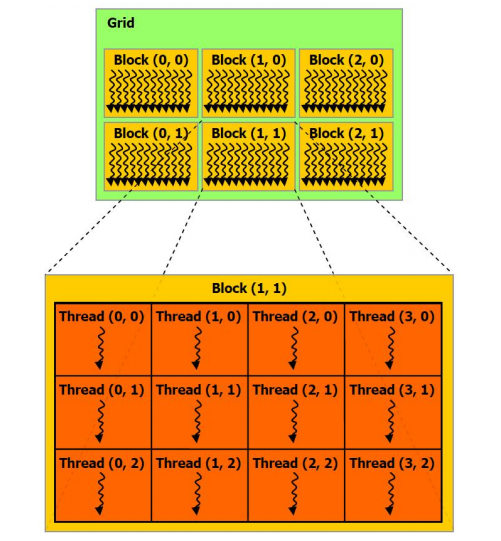
\includegraphics[scale=0.55]{images/cuda1.png}
	\caption{Organisierung von Threads in Blocks in Grids \cite{cud2012}}
	\label{img:cuda1}
\end{figure}

\subsection{Speicherverwaltung}
\label{cudaMemory}

Dadurch, dass die Daten vom \textit{host} zum \textit{device} kopiert werden müssen und vice versa, unterscheidet cuda zwischen \textit{host memory} und \textit{device memory}. Darüber hinaus ist der \textit{device memory} bereits auf der Grafikkarte in verschiedene Bereiche organisiert, wie in Abbildung \ref{img:cuda_mem} dargestellt. Jeder Multiprozessor hat Zugriff auf den \textit{global memory} sowie einen eigenen lokalen \textit{shared memory}, \textit{Constant} und \textit{Texture Cache}. Lokal erstellten Variablen werden als \textit{Register} bezeichnet. Auf diese ist der Zugriff mitunter am schnellsten, jedoch sind sie lokal pro Thread. Die Daten liegen als Parameter zunächst im \textit{global memory} vor. Im \textit{Constant Cache} liegen alle durch das cuda Schlüsselwort \textit{\textunderscore\textunderscore constant\textunderscore\textunderscore} deklarierte Werte. Zugriffe auf den \textit{global memory} sind am langsamsten, da der Speicherbereich zwischen allen Multiprozessoren geteilt wird und Zugriffe mitunter synchronisiert werden müssen \todo{HARDWARE}. Durch Verwendung des \textit{shared memory} und \textit{texture cache} können Speicherzugriffe beschleunigt werden, jedoch können Daten aus diesen Bereichen nicht zwischen Blöcken geteilt werden.

\begin{figure}
	\centering
	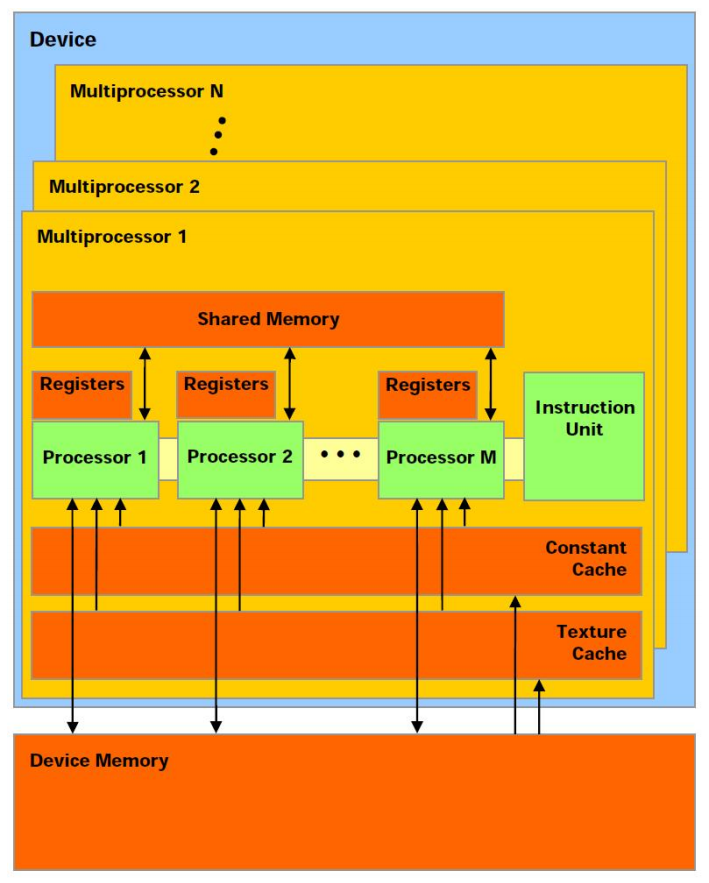
\includegraphics[scale=0.4]{images/cuda_mem.png}
	\caption{Organisierung der verschiedenen Speichertypen}
	\label{img:cuda_mem}
\end{figure}

\subsubsection{Shared Memory}

Gerade bei vielen parallelen Lese- / Schreibzugriffen kann hier eine hohe Latenz auftreten, wenn viele Threads auf die gleichen Adressen zugreifen. Aus diesem Grund empfiehlt es sich, die benötigten Daten von dem \textit{global} in den \textit{shared memory} zu kopieren. Der \textit{shared memory} wird von allen Threads in einem Block geteilt. Beim Kopieren der Daten muss ein Index berechnet werden, um die korrekten Daten dem jeweiligen Block zuzuordnen. Weiterhin ist zu beachten, dass nicht beliebig viel \textit{shared memory} allokiert werden kann: Je nach Grafikkarten stehen pro Block zwischen 16 und 48 Kilobyte Speicher zur Verfügung. 

\todo{Ausführlicher}

\subsection{Vektor Addition}

Am Beispiel der Vektor Addition soll der Aufbau und Ablauf eines cuda Programms illustriert werden. Hierfür wird zunächst die Funktion \textit{vecAdd} angelegt. Hier wird in Zeile 8 - 10 durch \textit{cudaMalloc} der benötigte Speicher für die Vektoren und das Ergebnis allokiert. Anschließend werden die Daten von Vektor $a$ und $b$ zum \textit{device} kopiert. In den beiden folgenden Zeilen wird der Inhalt der Vektoren $a$ und $b$ vom \textit{host} zum \textit{device} kopiert. In Zeile 15 wird der \textit{kernel} \textit{add} aufgerufen, der auf der Grafikkarte ausgeführt wird. Einem \textit{kernel} muss durch Angabe in den dreifachen spitzen Klammern, die Dimension des Grids und der Blocks mitgeteilt werden. Im Beispiel werden pro Block 256 Threads verwendet (\textit{numThreads}) und die Anzahl der notwendigen Blocks aus der Vektorgröße und der Threadanzahl berechnet. Da die Verarbeitung asynchron erfolgt, wird durch \textit{cudaDeviceSynchronize} in der nächsten Zeile die Ausführung auf dem \textit{host} pausiert, bis die GPU fertig ist. In Zeile 17 wird das Ergebnis vom \textit{device} zurück zum \textit{host} kopiert und kann ausgegeben oder weiterverarbeitet werden.
Der \textit{kernel} wird von jedem Thread ausgeführt. Jeder Thread kümmert sich um die Addition eines Elementes aus $a$ und aus $b$ am selben Index. Damit dieser Index global eindeutig ist, muss neben der $threadId$ in x-Richtung die Grid und Blockdimension des Threads berücksichtigt werden. Falls der berechnete Index innerhalb der Vektoren liegt, wird die Summe in $c$ geschrieben.

\lstset{language=C}
\begin{lstlisting}
void vecAdd (float *a, float *b, float *c, int size) {
	int numThreads = 256;
	int numBlocks = (size + numThreads - 1) / numThreads;
	float *aPtr = 0;
	float *bPtr = 0;
	float *cPtr = 0;	
	
	cudaMalloc((void **) aPtr, a, sizeof(float) * size);
	cudaMalloc((void **) bPtr, b, sizeof(float) * size);
	cudaMalloc((void **) cPtr, c, sizeof(float) * size);	
	cudaMemcpy(aPtr, a, sizeof(float) * size, cudaMemcpyHostToDevice);
	cudaMemcpy(bPtr, b, sizeof(float) * size, cudaMemcpyHostToDevice);	
	
	add<<<numBlocks, numThreads>>>(aPtr, bPtr, cPtr, size);
	cudaDeviceSynchronize();
	
	cudaMemcpy(c, cPtr, mem, cudaMemcpyDeviceToHost);
	
	cudaFree(aPtr);
	cudaFree(bPtr);
	cudaFree(cPtr);
}

__global__ void add (float *a, float *b, float *c, int size) {
	int id = blockDim.x * blockIdx.x + threadIdx.x;
	if (id < size) c[id] = a[id] + b[id];
}
\end{lstlisting} 

